\documentclass[../psets.tex]{subfiles}

\pagestyle{main}
\renewcommand{\leftmark}{Problem Set \thesection}
\setcounter{section}{4}

\begin{document}




\section{Group Structure Applications}
\begin{enumerate}
    \item \marginnote{11/7:}Automorphisms of $S_n$.
    \begin{enumerate}
        \item Let $\psi:G\to G$ be an isomorphism. If $\{c\}$ is a conjugacy class of $G$, prove that the image $\psi(\{c\})$ of $\{c\}$ under $\psi$ is the conjugacy class $\{\psi(c)\}$.
        \item Deduce that $|\{c\}|=|\{\psi(c)\}|$.
        \item Let $G=S_n$. Prove that $|\{(1,2)\}|=n(n-1)/2$.
        \item If $n\neq 6$ and $\sigma\in S_n$ has order 2, prove that $|\{\sigma\}|=|\{(1,2)\}|$ if and only if $\sigma$ is a 2-cycle.
        \item Deduce that if $\psi:S_n\to S_n$ is an isomorphism and $n\neq 6$, then $\psi$ takes 2-cycles to 2-cycles.
        \item Suppose that $\psi[(1,2)]=(i,j)$. Prove that, after possibly swapping $i$ and $j$, $\psi[(1,3)]=(i,k)$ for some $k\notin\{i,j\}$.
        \item Let $g\in S_n$ denote any element with $g(i)=1$, $g(j)=2$, and $g(k)=3$. Let $\phi_g$ be the (inner) automorphism of $S_n$ given by conjugation by $g$. After replacing $\psi$ by $\phi_g\circ\psi$, deduce that one can assume that $\psi[(1,2)]=(1,2)$ and $\psi[(1,3)]=(1,3)$.
        \item Assume that $\psi(1,i)=(1,i)$ for all $i<k$ with $k>3$. Prove that $\psi(1,k)=(1,j)$ for some $j\geq k$. As in part (g), show that after replacing $\psi$ by $\phi_h\circ\psi$ for some $h$, one can assume in addition that $\psi[(1,k)]=(1,k)$.
        \item Deduce that $\psi$ is the identity, and hence that any automorphism of $S_n$ (for $n\neq 6$) is given by conjugation, i.e., $\Out(S_n)=1$ for $n\neq 6$.
    \end{enumerate}
    \item Let $H$ be a finite subgroup of $G$ of index $n$. Let $A$ be the set of left cosets $G/H$, and consider the left action of $G$ on $A$. (See Exercise 4.2.8 of \textcite{bib:DummitFoote}.)
    \begin{enumerate}
        \item Let $n=|G/H|$, and consider the associated homomorphism $G\to S_{G/H}\cong S_n$. Prove that the kernel of this map is a subgroup of $H$.
        \item By considering the kernel of the map $G\to S_n$, deduce that $G$ contains a normal subgroup $N$ contained in $H$ of index dividing $n!$ and divisible by $n$.
    \end{enumerate}
    \item Let $\text{Do}\cong A_5$ denote the symmetry group of the dodecahedron. Fill out the missing entries in the table below for various sets $X$ on which $\text{Do}$ acts transitively. Since the action of $\text{Do}$ is transitive for each $X$, all stabilizers $S$ for any point $x\in X$ are conjugate to the stabilizers of any other point. Hence, they are isomorphic as subgroups; simply list a group (from our known list of groups: symmetric, alternating, dihedral, cyclic, quaternion, etc.) isomorphic to any of the stabilizers.
    \begin{center}
        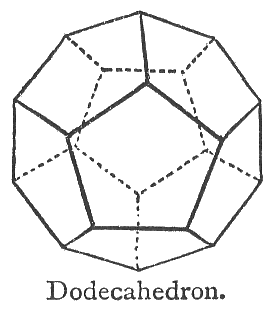
\includegraphics[width=0.18\linewidth]{../ExtFiles/Dodecahedron.png}
    \end{center}
    \begin{proof}
        {\color{white}hi}
        \begin{center}
            \small
            \renewcommand{\arraystretch}{1.2}
            \begin{tabular}{|l|l|l|l|l|}
                \hline
                $X$ & $|X|$ & Faithful? & $\Stab(x)$ & $|S|$\\
                \hline
                Dodecahedra & 1 & No & $S=\text{Do}\cong A_5$ & 60\\
                Inscribed cubes &  &  &  & \\
                Pairs of opposite faces &  &  &  & \\
                Faces &  &  &  & \\
                Vertices &  &  &  & \\
                Edges &  &  &  & \\
                \hline
            \end{tabular}
        \end{center}
    \end{proof}
\end{enumerate}




\end{document}